\documentclass[letterpaper,12pt,titlepage,fleqn]{article}

\setlength{\mathindent}{1cm}

\usepackage{graphicx}                                        

\usepackage{amssymb}                                         
\usepackage{amsmath}                                         
\usepackage{amsthm}                                          

\usepackage{alltt}                                           
\usepackage{float}
\usepackage{color}

\usepackage{url}

\usepackage{balance}
\usepackage[TABBOTCAP, tight]{subfigure}
\usepackage{enumitem}
\usepackage{mathptmx}
\usepackage{epsfig}
\usepackage{pstricks, pst-node}

\usepackage{cite}
%\usepackage{indentfirst}
\usepackage{listings}
\usepackage{CJK}
\usepackage{url}
\usepackage{setspace}
\onehalfspacing

% the following sets the geometry of the page
\usepackage{geometry}
\geometry{textheight=9in, textwidth=6.5in}

% random comment

\newcommand{\cred}[1]{{\color{red}#1}}
\newcommand{\cblue}[1]{{\color{blue}#1}}

\usepackage{hyperref}

\usepackage{textcomp}
\usepackage{listings}
\def\name{Reza Ziazi \\ \\Yu Zhang}

%% The following metadata will show up in the PDF properties
\hypersetup{
  colorlinks = true,
  urlcolor = black,
  pdfauthor = {\name},
  pdfkeywords = {CS 519 Final Project},
  pdftitle = {CS 519 Final Project},
  pdfsubject = {CS 519 Final Project},
  pdfpagemode = UseNone
}

\parindent = 0.0 in
\parskip = 0.2 in

\title{CS 519 Final Project\\Vector Analysis for Flow Visualization in a Turbulent Porous Media}
\author{\name}

\begin{document}

\maketitle

\setlength{\parindent}{2em} 

\begin{CJK}{UTF8}{gkai}

\section{Abstract}
An experimental method has been applied to the study of turbulent flow in porous media to detect the complex vortical structures in the complicated geometries  which are interesting to be visualized. This study compares the visualization methods based on the results of Particle Image Velocimetry (PIV) technique which are obtained using refractive index matched data of PIV. A detailed velocity vector field is investigated using three different visualization techniques such as swirl strength, second invariant Q, and . The flow visualization technique is based on the line integral convolution, and color mapping of the flow field. 
\section{Introduction}
Porous media flows have been emerged to be very influential and widely used in diverse scientific researches, as well as industrial and environmental disciplines in recent years as it attracted considerable research interest. Numerous applications such as chemical and catalytic reactors, geology, oil, gas and geothermal reservoirs, reactive fluid flow in fractures, sediment transport, advanced heat exchangers and filters, chromatography columns, groundwater hydrology, polymer brushes, fluid flow in biological systems, and heat pipe technology are representatives of the high level interest in studying the fluid mechanics of flow through porous media. The significance of the issue and the complex mechanism have been combined to provoke a desire to do research in two parts: experimental and computational fluid mechanics in the pores. 
Some of the early contributions in the field of characterization of the flow in porous media as has been proposed by Biot [1] models the porous media as a structural matrix that has been coupled with the fundamentals of creeping flows in the pores, which is governed by Darcy’s law. This pioneered perspective of porous media has been frequently used in the general field of poromechanics. As a complementary fluid mechanic prospect to the Biot’s solid-fluid coupled hypothesis, some detailed and basic studies of  fluid mechanics of porous media was introduced by Bear [2], Scheidegger [3], and others who provided basic relationships and parameters of the physics of this type of multiphase flows. Hence, the essence of investigating the behavior of fluid flow in porous media requires both experimental and computational study in a simplified apparatus, which facilitates the experimental elusions, and computational constraints associated with the physics of porous media flows, which is discussed.\\
\\
Fluid mechanics of porous media has been scrutinized based on the pore scales (microscopic and macroscopic) by implementing invasive and non-invasive experimental methods to validate the computational methods. Almost most of those experimental methods employed to study porous media have implemented the optical techniques which can be either invasive or non-invasive.  These non-intrusive methods are classified as (1) Particle Image Velocimetry(PIV) [4-8,30], (2) Particle Tracking Velocimetry (PTV) [9-11], (3) Laser-Induced Fluorescence (LIF) [12,13], (4) Laser Doppler Anemometry (LDA) [14,15], (5) Magnetic Resonance Imaging(MRI) [16, 17], and X-ray Computed Tomography (XCT) [18]. PIV method has the advantage of being used for the for instantaneous velocity measurement, although reflects some weaknesses for investigating the flow around glass beads. The justifications beyond using PIV rather than other visualization techniques depend on many elements where some of them are fruitful to be mentioned in this analysis. Other methods such as MRI and XCT are capable of being used in certain flow situations for the case of opaque materials. In this study, PIV has been chosen as the experimental method to visualize the flow field in the pores around the spheres. In this study, a PIV setup for capturing the instantaneous velocities is being developed. The limitations are (1) elusiveness of optical interrogation access, (2) distortion of the light within the media, and (3) refractive index mismatch (RIM) which are minimized to make the bed ready to transmit the optical rays and without distortion. Bed aspect ratio which is the length of the bed to the diameter of the beads (L/DB) is important when the effects of near wall region are to be considered. In the following study, the aspect ratio of the bed is chosen to be low and the flow regime represents a creeping flow.

\section{PIV Method and Experimental Apparatus}

Pore scale experiments of porous media flows are confined to non-invasive approaches due to lack of ability to measure the pore scale velocities without disturbing the flow field. PIV is the method that has been used for several similar applications. The specification of the experimental setup is summarized in Table 1. 
\clearpage

\begin{table}[!h]
	\centering
	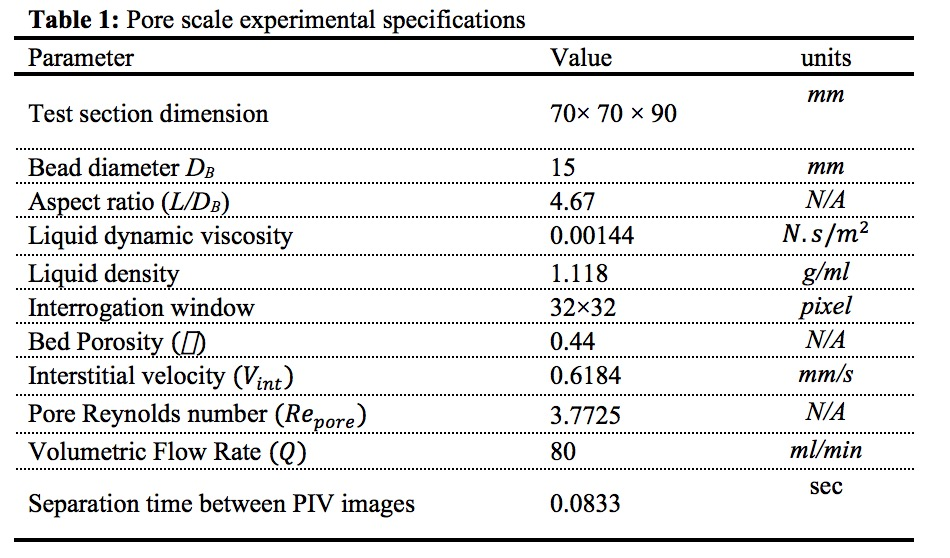
\includegraphics[width=\linewidth]{Pore.jpg}
	\caption{Pore scale experimental specifications}
\end{table}

The procedure to accomplish a PIV measurement include (a) data acquisition, (b) pixelization, (c) interrogation, (d) validation, and (e) final results.



\begin{figure}[!h]
	\centering
	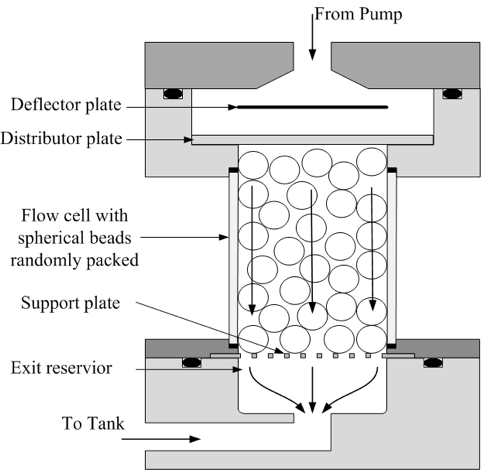
\includegraphics[width= 0.5\linewidth ]{pump.png}
	\caption{Schematic of PIV test facility test section}
	
\end{figure}
The pore Reynolds number is evaluated based on the interstitial velocity which is the pore-scale velocity.
\begin{figure}[h]
	\centering
	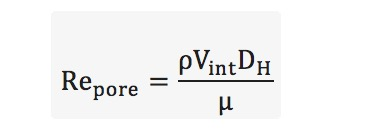
\includegraphics[width= 0.3\linewidth ]{eq.jpg}	
\end{figure}
\\where, Vint is the interstitial velocity, and DH is the pore-scale  hydraulic diameter that is defined using the following relation: 
\begin{figure}[h]
	\centering
	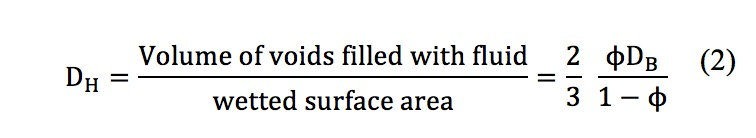
\includegraphics[width= 0.5\linewidth ]{eq2.jpg}	
\end{figure}
\\Ammonium Thiocyanate (NH4SCN) is the working fluid for this experiment which has a dynamic viscosity of 0.00144  . As it is depicted in Figure 1, the experiments were carried out in a test section which has been designed for the current study. This experimental setup designed for PIV measurement in the proposed paper consists of a main test section transparent to the camera made from Pyrex (70mm  70mm  90 mm long) that was randomly packed with 15 mm diameter Pyrex beads. Therefore, the aspect ratio of the bed is 4.67. According to the proposed experimental work performed by Patil and Liburdy [30], the imaging system was based on pulsed lighting from a Nd-YLF laser at 527 nm (New Wave Research, Pegasus PIV) and a CMOS camera (Integrated Design Tools Inc. Model MotionProTM X-3).

\section{Data deduction and processing}
In order to assure proper comparison of results factors such as sphere position, volume fraction, and the near wall region need to be evaluated. The effect of these on both the experimental data and the simulation results are discussed in this section. 
The sphere position was determined by looking at changes in diameter of glare off bead surfaces. The image degradation (can be also known as aberration) in solid liquid interfaces emanating from different refracting powers (refractive index effects), which is a result of slight surface refraction on the aforementioned interfaces that may cause a PIV bias error. The diameter of glare edges was determined by fitting a circular tool in IMAGEJ using an edge detection method [28, 29].
Collecting PIV data is restricted to the interrogation window, therefore, since the resolution is determined by the interrogation window size, collecting data very close to solid-liquid wall is not possible especially with the problem mentioned for the glare (noise) off the bead surface. So, when the solid region occupying more than certain critical percent of interrogation window area, the data was discarded. The critical value used is generally 50\%. Because of the mentioned optical issues to measure the velocities with a clear PIV image near the wall region, a representative square slice region (30mm×30mm) was chosen based on the geometry and interests of flow physics. The data analyzed in this paper are all in this region. Flow regions closer than 20 mm away from the wall have been removed, therefore the horizontal domain ranges from X = -0.015 (m) to X = 0.015 (m). In the vertical direction, to diminish the impact of the upstream entrance on the flow field inside the test section, a section ranging from Y = -0.01 (m) to Y = 0.02 (m) was used. All of the results are shown in the z-plane (Figure 2), where z/DB=0.43.

\begin{figure}[!h]
	\centering
	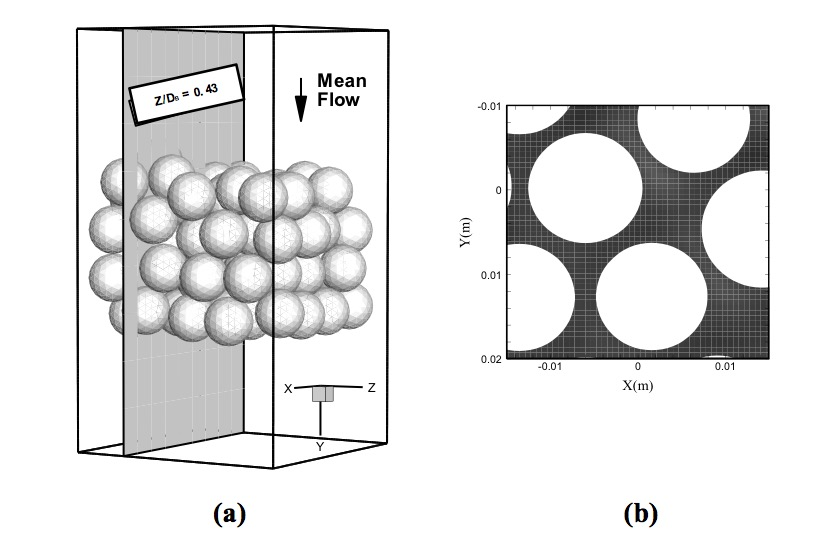
\includegraphics[width= 0.5\linewidth ]{pic2.jpg}
	\caption{Geometry of flow field (a) the whole domain in three dimension, (b) the two dimensional sub-region inside the flow field.}
\end{figure}

\section{Methods of Visualization}
The local behavior of the vector field can be approximated by computing a local stream line that starts at the center of pixel (x, y) and moves out in the positive and negative directions.
Let u be the vector field. Then a streamline parametrized by arc length can be defined as:

\begin{figure}[!h]
	\centering
	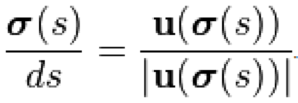
\includegraphics[width= 0.2\linewidth ]{pic3.png}

\end{figure}

Let
\begin{figure}[!h]
	\centering
	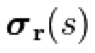
\includegraphics[width= 0.05\linewidth ]{pic4.png}

\end{figure}
 \\ be the streamline that passes through the point r for s = 0. Then the image color can be set to 

\begin{figure}[!h]
	\centering
	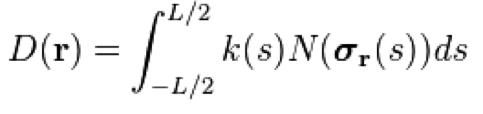
\includegraphics[width= 0.5\linewidth ]{pic5.png}
\end{figure}

\textbf{Macro Field}
\begin{figure}[!h]
	\centering
	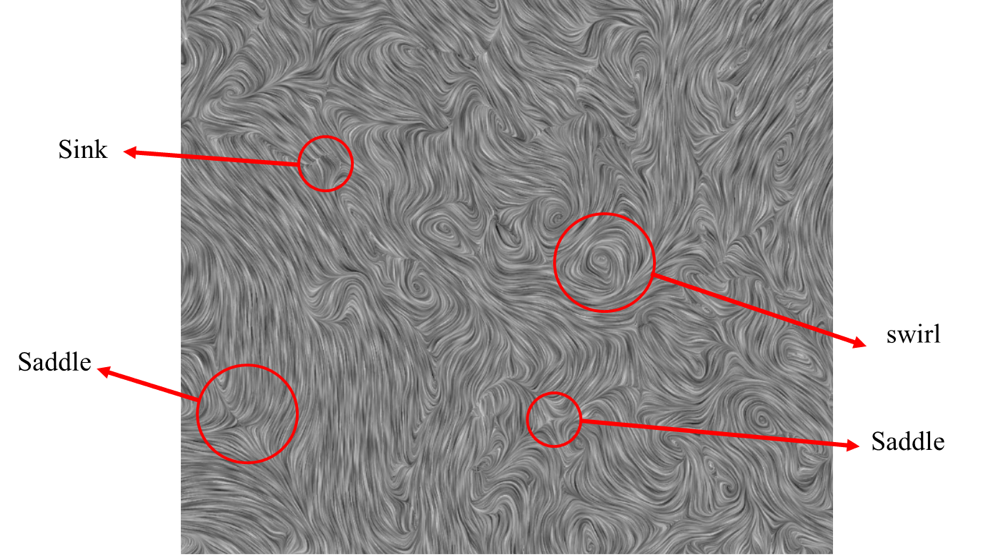
\includegraphics[width= 0.7\linewidth ]{pic6.png}
\end{figure}

\textbf{Micro Field}
\begin{figure}[!h]
	\centering
	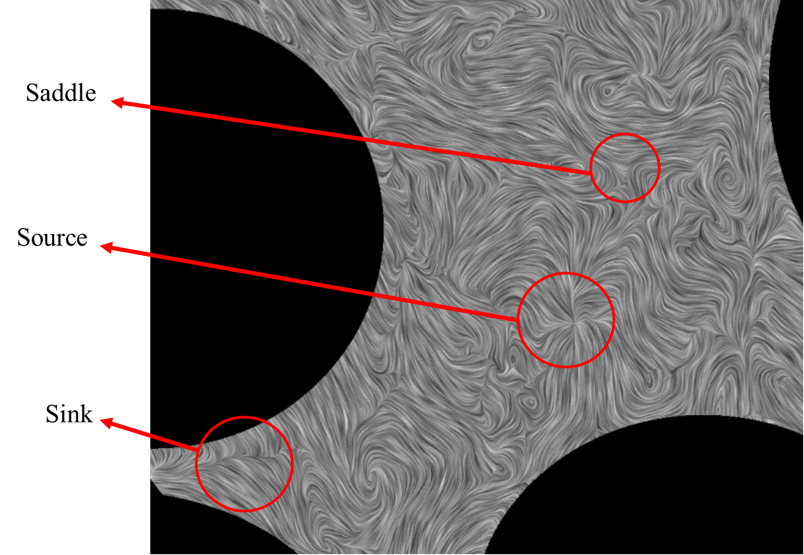
\includegraphics[width= 0.5\linewidth ]{pic7.png}
\end{figure}

\section{Methods of Vortex detection}
\begin{enumerate}
\item \textbf{$\lambda_{ci}$ Method}\\
Swirling strength is defined as the imaginary part of the complex eigen value of the velocity gradient tensor J:
\begin{figure}[!h]
	\centering
	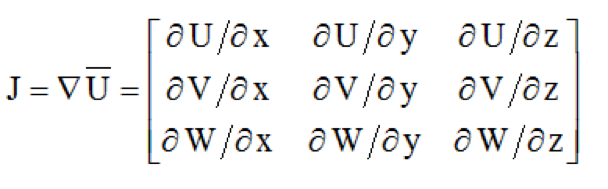
\includegraphics[width= 0.5\linewidth ]{pic8.png}
\end{figure}
\\For planar data gradients in the z-direction cannot be calculated, and setting them to zero simplifies eigen value calculation, so the square of the imaginary part can be computed as:
\begin{figure}[!h]
	\centering
	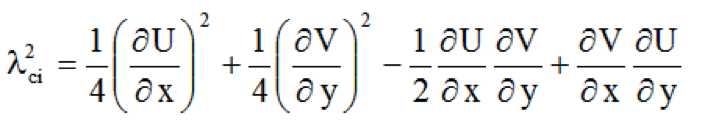
\includegraphics[width= 0.5\linewidth ]{pic9.png}
\end{figure}
\\Local minima of negative-valued swirling strength can be used to identify vortex cores, while positive values indicates areas of the flow, where shear may be present, but no swirling motion..
\begin{figure}[!h]
	\centering
	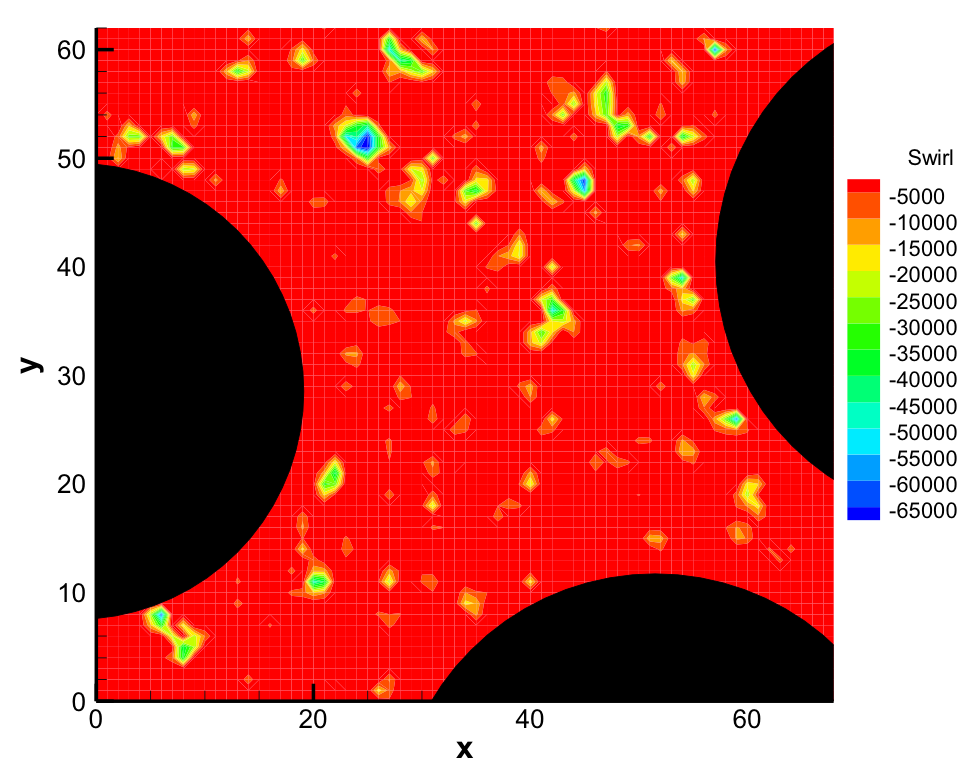
\includegraphics[width= 0.5\linewidth ]{pic10.png}
\end{figure}

\item \textbf{2nd Invariant Q}\\
The 2nd invariant Q of the 3x3 velocity gradient matrix J may also be used to identify vortices. The full gradient matrix J can be described as:\\
\begin{figure}[h]
	\centering
	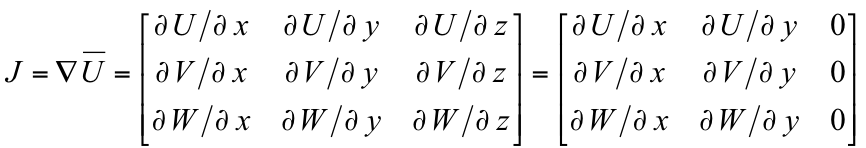
\includegraphics[width= 0.8\linewidth ]{pic11.png}
\end{figure}
\begin{figure}[h]
	\centering
	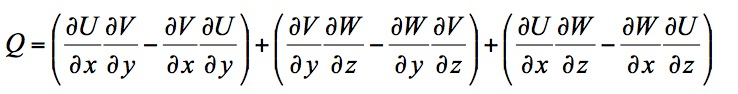
\includegraphics[width= 0.8\linewidth ]{pic12.jpg}
\end{figure}
\\In the immediate vicinity of a vortex Q will be positive and have a maximum at the vortex core. Local maxima of positive Q can be used to identify vortex cores, while negative values indicates areas of the flow, where shear may be present, but no swirling motion.

\begin{figure}[h]
	\centering
	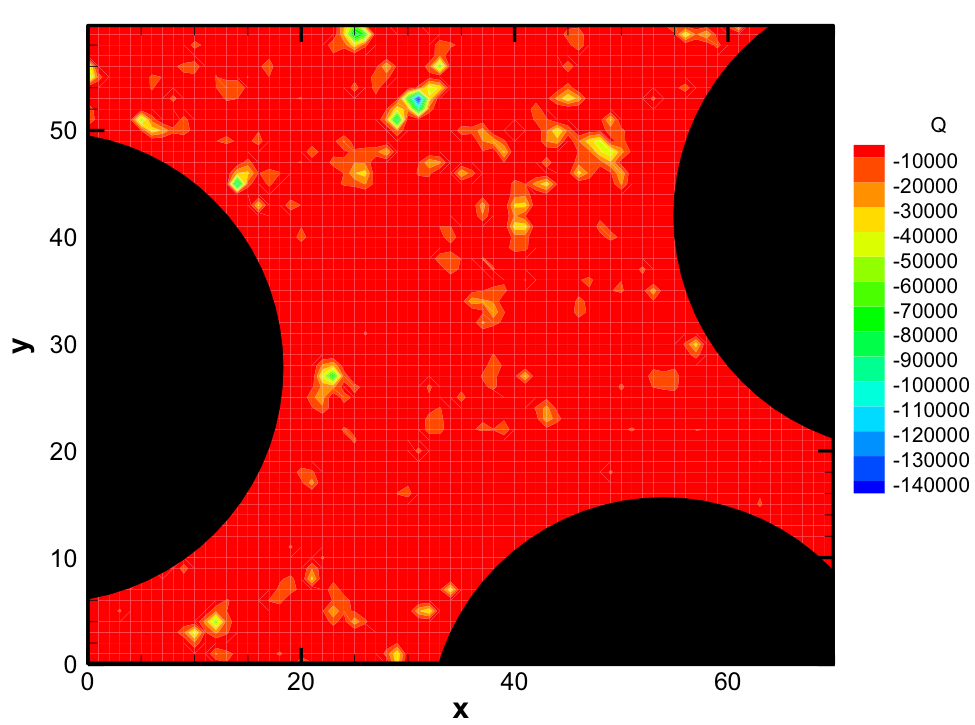
\includegraphics[width= 0.8\linewidth ]{pic13.png}
\end{figure}

\end{enumerate}

\section{Implementation of Visualization}
In this part, for making the real data be visualized, I will introduce how we analyze the dataset, how we make LIC visualization with the dataset, and how we use color mapping to explore our data deeper. 

\begin{enumerate}
\item \textbf{Dataset Analysis}\\
As before mentioned, the data is recorded as the movement that flow goes through a group of sphere. And in this part, we will introduce the dataset.\\
There are 79 * 63 points in the original dataset which includes, x, y, x(pix)(pix), x(mm)(mm), U pix[pix], V pix[pix], U[m/s], V[m/s], Length[m/s], and Status. 

\begin{table}[!h]
	\centering
	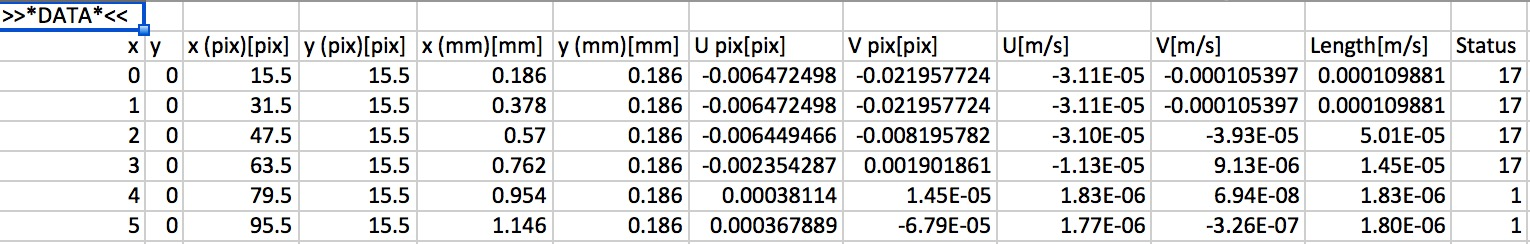
\includegraphics[width=\linewidth]{data1.jpg}
	\caption{Raw dataset}
\end{table}

We need to find out which elements are matched up with our requirements. According to the discussion in our group, we decided to use the following elements: x, y, U[m/s], V[m/s], Length[m/s] and Status. Among them, U[m/s] means the velocity in X axis direction and U[m/s] means the velocity in Y axis direction; Length[m/s] means the magnitude of the velocity; Status is used to filter the data.\\
So after subtracting data, we got the dataset that we can used in our implementation as following:
\begin{table}[h]
	\centering
	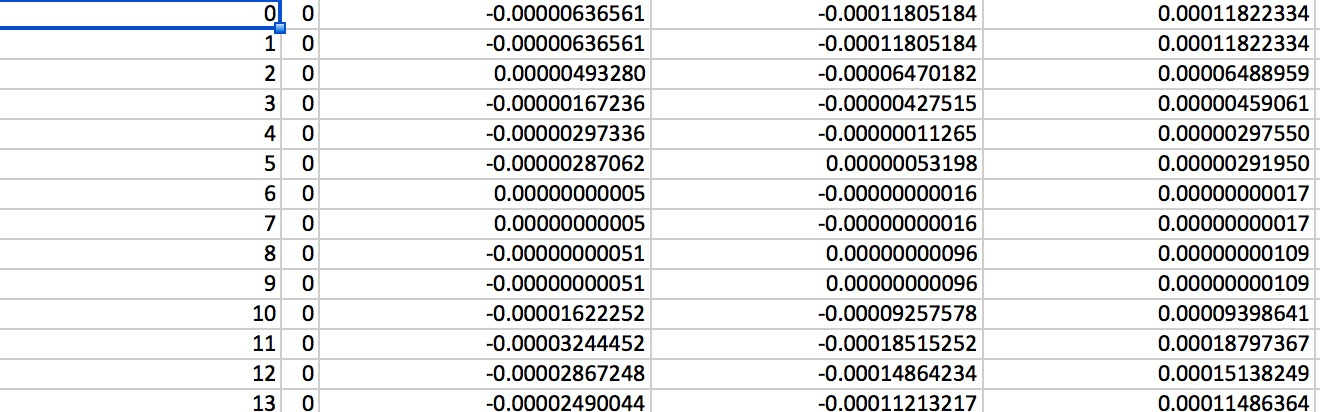
\includegraphics[width=\linewidth]{data2.jpg}
	\caption{Filtered dataset}
\end{table} \\
The new dataset contains 79 * 63 points and each point has its U velocity, V velocity, the magnitude of the vector’s velocity, and its own status. It is apparently to see that our data belongs to vector filed.
The status value may be confusing when you first time to see it. But it is an important factor to subtract our data. As we mentioned before, there are a bunch of spheres existing while flow going through. And by my partner Reza introducing, the flow in one sphere can be treated as “trash information”, it cannot help us to see how the exact flow moves so that we need to filter this “trash information” off.

\item \textbf{Programming Methods Analysis}
By learning and analyzing our dataset, we decide to use LIC and color mapping to make the data visualized. The reasons for this are:
    1) LIC visualization is a good way to see the movement of vectors at one specific time.\\
    2) LIC visualization has already been implemented in Project2. One hand we are familiar with it; on the other hand, in our Project2, there’s still some small problem existing, and this is a good chance for us to modify the algorithm and check if it correct by the real data.\\
    3)Color mapping is a useful way to see how fast flows move at one specific time. We use the Rainbow Color Mapping idea to make color mapping visualization.\\
For coding the program, luckily I have started learning OpenGL this term by taking CS 553 which is Scientific Visualization. So I use OpenGL by C++ language to code the program.\\
In our program, there are mainly parts being necessary to concern.\\
1) Texture mapping the data to the static 2D geometry. We use interpolation to accomplish, and the function call is\\
 interpolating (double ** vectorField, double ** scalarField, int ** v\_status)\\
In this function, I filter our data here by parameter v\_status: \\
 if(v\_status[m][n] ==0 $\lVert$ v\_status[m][n] == 16)\{\\
	  flowVector[2 * index] = v\_x;\\
	  flowVector[2 * index + 1] = v\_y;\\
\}\\
This means we only need the data with status 0 and status 16. In other word, status 17, 1 mean the relative vectors are in the sphere that contains “trash information” \\

2) Implementing LIC algorithm. The basic equation is
\begin{figure}[h]
	\centering
	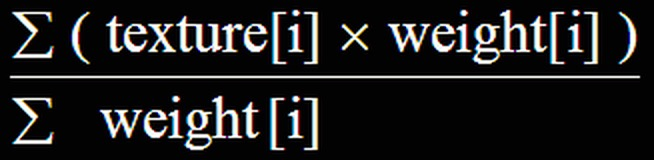
\includegraphics[width=0.5\linewidth]{LIC.jpg}

\end{figure}

And what I really want to mention is that to implement LIC visualization, we need to not only calculate the only one direction’s (such as the positive direction) streamline, but also the opposite direction’s (such as the negative direction) streamline. This is why I did wrong in our Project2.\\

3) Color mapping scale defining. In our implementation, we define that from Blue to Red means from low velocity to high velocity. This means that faster the velocity is, the brighter Red you can see.

\item \textbf{Results Presentation and Analysis}\\
\textbf{LIC Visualization}\\
\begin{figure}[htbp]
	\centering
	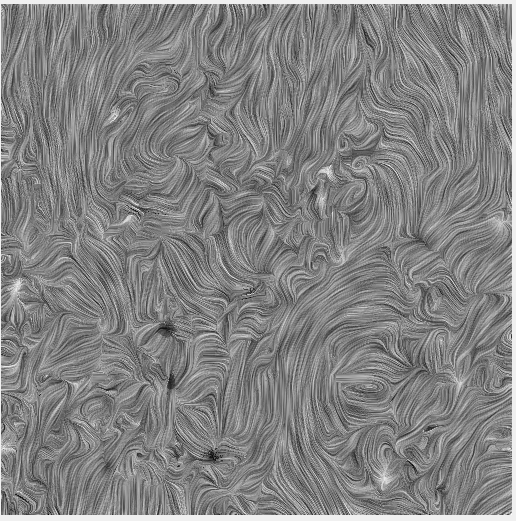
\includegraphics[width=0.4\linewidth]{image/raw8.png}
		\caption{LIC of Raw dataset}
\end{figure}
As you can see Figure 3, it is from the Raw dataset, there's a lot of noise, and it cannot offer us much useful information.\\
\begin{figure}[htbp]
	\centering
	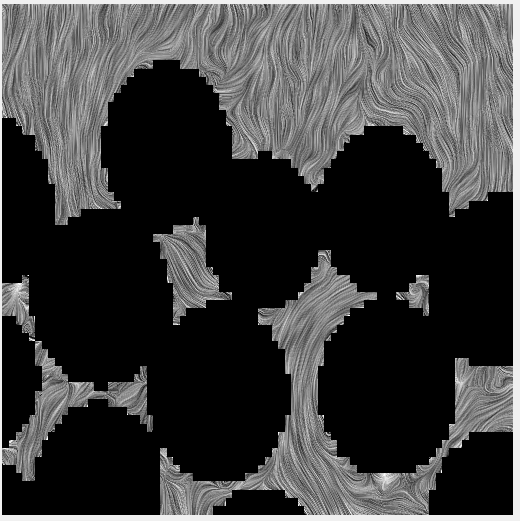
\includegraphics[width=0.4\linewidth]{image/v8.png}
		\caption{LIC of filtered dataset}
\end{figure}
The figure 4 shows the data that being filtered, and the black part is the spheres. This means the data is filtered and it is more easily to see how flows move between spheres. \\
\begin{figure}[htbp]
	\centering
	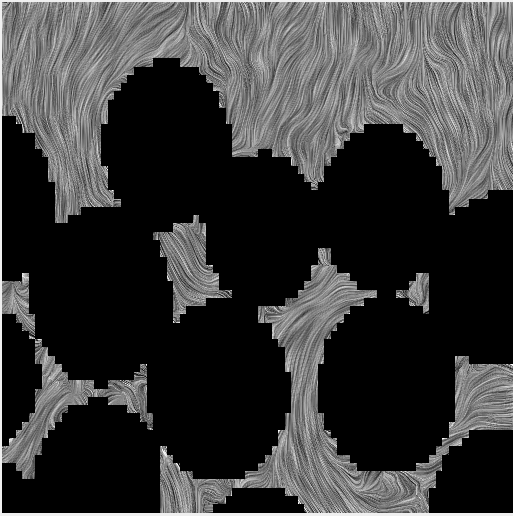
\includegraphics[width=0.4\linewidth]{image/v16.png}
		\caption{LIC of filtered dataset in different time}
\end{figure}

\clearpage
\item\textbf{Color Mapping Visualization}\\
\begin{figure}[htbp]
	\centering
	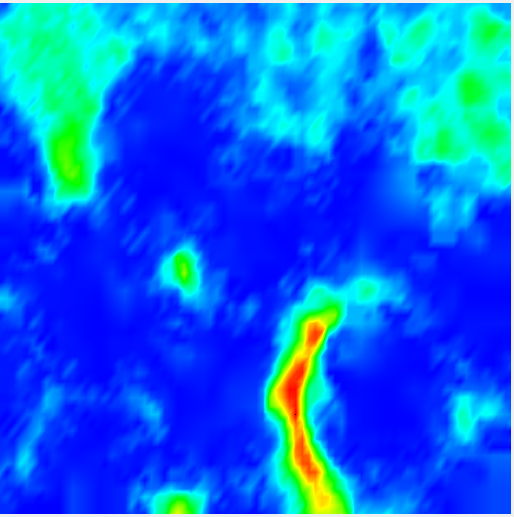
\includegraphics[width=0.4\linewidth]{image/colorv8.png}
		\caption{LIC of RAW Dataset}
\end{figure}
In the color mapping, it is enough to use raw dataset, and it is also a useful way to help us to see the spheres part. As you can see, in the middle of the figure, there are several round deep blue parts which represent Sphere. I think it is the way that can prove our LIC visualization is right.\\
At the same time, you can see there are some brighter parts, this means that the flow in these parts have higher speed. When you check Figure 5, you can also see the same effects.\\

\begin{figure}[htbp]
	\centering
	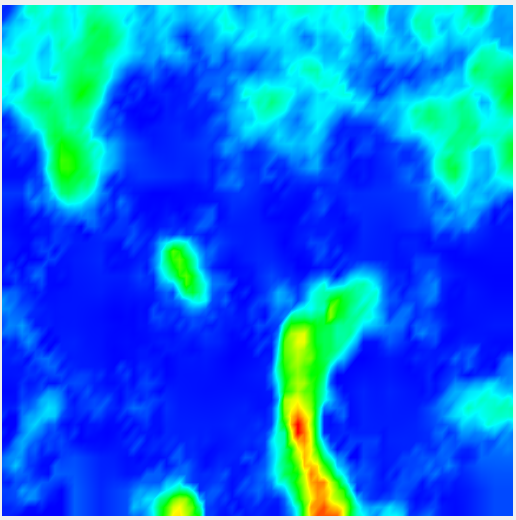
\includegraphics[width=0.4\linewidth]{image/colorv16.png}
		\caption{LIC of Raw Dataset in Different Time}
\end{figure}
\end{enumerate}

\clearpage
\section{Conclusion and Comments of CS 519 Final Project}
\begin{enumerate}
\item In this project, we learned several relevant methods to handle vector field. And I also learned some knowledge about physics. I think it is really important for me because it is my first time to apply the real data into visualization. It means a lot to me.\\
\item For theroies about Tensor field, I think our future job should focus on this. Since Vector has its own limitation, if we want to learn more about vectors, we need to use Tensor filed theroies.\\
\item My personal view is that, in our project, LIC and Color Mapping are two useful and relevant way to visualize the data, they can prove each other right or wrong. And we can easily disdinguish the characters of each timestep's view.\\
\item This Latex file is made by myself, since there's not much time for me, I am really sorry about the format. Hopefully people can enjoy it.
\item Finally, I have some personal comments for this project. Teamwork is really important in our study life. And it is my first time to work with a Ph.D. student, it is a really good chance to learn more things. Although there were some little misunderstanding, and kind of wasting time. But finally we solved the problem, and implement things we want to see. This class teach me really really lots of things. Thanks to Professor Zhang, and thanks to my partner Reza.

\end{enumerate}
\clearpage
\section{Reference}
1	Biot, M. A. (1941). “General theory of three dimensional consolidation”. Journal of Applied Physics, 12(2), 155–164.
2	Bear, J. (1972). Dynamics of fluids in porous media. Elsevier. \\
3	Scheidegger, A. E. (1974). The physics of flow through porous media. Universty of Toranto Press.\\
4	Patil, V. a., and Liburdy, J. a. (2013). “Flow characterization using PIV measurements in a low aspect ratio randomly packed porous bed”. Experiments in Fluids, 54(4), 1497.\\
5	Arthur, J. K., Ruth, D. W., and Tachie, M. F. (2009). “PIV measurements of flow through a model porous medium with varying boundary conditions”. Journal of Fluid Mechanics, 629, 343.\\
6	Northrup, M. A., Kulp, T. J., Angel, S. M., \& Pinder, G. F. (1993). “Direct measurement of interstitial velocity field variations in a porous medium using fluorescent-particle image velocimetry”. Chemical Engineering Science, 48(1), 13–21.\\
7	Saleh, S., Thovert, J. F., \& Adler, P. M. (1992). “Measurement of two-dimensional velocity fields in porous media by particle image displacement velocimetry”. Experiments in Fluids, 12(3), 210–212.\\
8	Hassan, Y. a., \& Dominguez-Ontiveros, E. E. (2008). “Flow visualization in a pebble bed reactor experiment using PIV and refractive index matching techniques.” Nuclear Engineering and Design, 238(11), 3080–3085.\\
9	Huang, A. Y. L., Huang, M. Y. F., Capart, H., \& Chen, R.-H. (2008). “Optical measurements of pore geometry and fluid velocity in a bed of irregularly packed spheres.” Experiments in Fluids, 45(2), 309–321.\\
10	Lachhab, A., Zhang, Y.-K., \& Muste, M. V. I. (2008). “Particle tracking experiments in match-index-refraction porous media.” Ground Water, 46(6), 865–72.\\
11	Cushman, J. H., \& Moroni, M. (2001). “Statistical mechanics with three-dimensional particle tracking velocimetry experiments in the study of anomalous dispersion. I. Theory.” Physics of Fluids, 13(1), 75.\\
12	Fontenot, M. M., \& Vigil, R. D. (2002). “Pore-scale study of nonaqueous phase liquid dissolution in porous media using laser-induced fluorescence.” Journal of Colloid and Interface Science, 247(2), 481–489.\\
13	Rashidi, M., Peurrung, L., Tompson, A. F. B., \& Kulp, T. J. (1996). “Experimental analysis of pore-scale flow and transport in porous media.” Advances in Water Resources, 19(3), 163–180.\\
14	Johnston, W., Dybbs, A., \& Edwards, R. (1975). “Measurement of fluid velocity inside porous media with a laser anemometer.” Physics of Fluids, 18(7), 913–914.\\


\bibliographystyle{plain}
\end{CJK}

\end{document}